\chapter{Discussion}
\label{section:discussion}
The main focus points during this thesis were the performance and stability of the algorithm. Most decisions were made with either performance or stability in mind, and often both. The performance and stability of the algorithm are discussed in section \ref{subsec:disc-perf} and \ref{subsec:disc-stab} respectively. Some important parameters and their impact on the algorithm are also discussen in \ref{section:imp-params}.
\section{Performance}
\label{subsec:disc-perf}
On the performance side, it is clear that the new algorithm with preprocessing is much faster than solving the pure MILP problem without preprocessing. Comparing the new algorithm to the pure approach is difficult since the challenging scenarios for the new algorithm simply cannot be solved with the pure approach.
\par
When it comes to scalability, there are a few noteworthy observations to make. 
\subsection{Path Length Scalability}
The first is that the time needed to solve each MILP subproblem does not depend on the length of the trajectory or the size of the world. Accounting for variations due to obstacle density, the average MILP solve times for scenarios using the same data set (San Francisco or Leuven) are very similar. Since the amount of segments scales linearly with the path length, the MILP part of the algorithm also scales linearly with the length of the initial path. This is in stark contrast with the exponential worst-case performance of the pure MILP approach.\\
However, this exponential complexity has not been eliminated. It has been shifted to the initial path planning algorithm: Theta*. This algorithm still has exponential worst-case complexity with respect to the length of the path. While Theta* does limit the scalability regarding the size of the world, it is a much easier problem to solve. It is part of the A* family of path planning algorithms which have been the subject of a large body of research.
\par
The algorithm separates the "routing" aspect from the trajectory planning aspect of the problem. The exact properties of the initial path are not very important. What matters is that it determines where and when to turn. By the time the MILP solver runs, the navigation aspect of the problem has already been solved. The MILP solver only needs to find a viable trajectory. The two aspects of the problem are solved separately, making both of them easier to tackle.
\par
The realization that these two aspects can be solved separately is the key insight that makes the performance improvements possible. Solving these aspects separately means that the optimal trajectory is unlikely to be found. However, at this point this seems like a necessary sacrifice for long term trajectory planning through complex environments. I could not find any algorithm in the literature that scales as well as my algorithm does, and is capable  of finding the optimal trajectory.

\subsection{Obstacle Density Scalability}
The second observation is that the density of the obstacles plays a large role in the scalability of the algorithm. The San Francisco and Leuven scenarios are very similar, except for their obstacle density. The Leuven scenario has a significantly higher density of obstacles and is also much harder to solve. Without preprocessing, the scalability of the MILP problem is limited by the total amount of obstacles. Because each MILP subproblem in my algorithm is roughly the same size, the total amount of obstacles is no longer the limiting factor. The density of the obstacles is the limiting factor in my algorithm.
\par
The Leuven scenarios can still be solved in an acceptable amount of time, but I do not believe this will be the case if the density is increased even more. Luckily, the Leuven data set is more detailed than it needs to be. Each building in the city is represented separately, even when multiple buildings are connected. It should be possible to reduce the obstacle density substantially with a minimal amount of effort. Figure \ref{fig:leuven-dense2} shows a dense region in the Leuven dataset where there is a lot of room for improvement.

\begin{figure}[h]
	\centering
	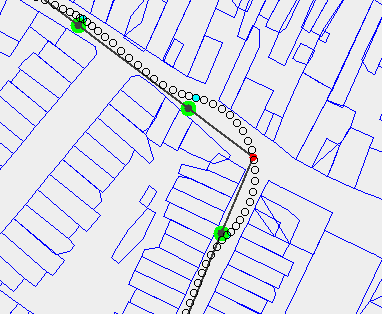
\includegraphics[width=0.5\textwidth]{leuven-dense}
	\caption{One of the denser regions in the Leuven dataset}
	\label{fig:leuven-dense2}
\end{figure}

Given that the Leuven data set is so unoptimized for this purpose and the algorithm still only needs, on average, a few seconds per segment, I believe that the scalability with regards to the obstacle density is acceptable.

\subsection{UAV Agility} 
The last observation is the importance of the agility of the UAV. The algorithm was developed with high-end consumer to professional grade multirotor UAVs in mind. These are very agile vehicles capable of impressive feats of acrobatics when properly piloted. This agility is one of the assumptions this algorithm is based on. The UAV must be able to hover and accelerate quickly.
\par
The results from the UAV agility experiment in section \ref{subsec:agility} show that these assumptions are indeed a critical part of the performance of the algorithm. The algorithm fails when faced with UAVs with an (unreasonably) low agility. 
\par
This reliance on agility is one of the factors that made the dramatic improvement in performance possible, but it also limits the applicability of the algorithm. However, the goal of this thesis was not to developed a general algorithm. The algorithm performs well for reasonable estimates of the agility of a multirotor UAV. On top of that, the agility of any UAV can be increased by limiting its maximum velocity\footnote{Limiting the maximum velocity of UAVs with a low acceleration when navigating through a city seems like a wise decision anyway. Such a UAV would not be able to react to unexpected obstacles quickly, so having it fly at a high velocity through the city seems like a dangerous proposition.}.


\section{Stability}
\label{subsec:disc-stab}
For the algorithm to be useful, it must be stable. The first aspect of stability is whether or not it can find a solution. If the algorithm is capable of finding a solution, it should find that solution every time. It should also be able to solve problems with a similar difficulty as well. The second aspect is that the solution for the same problem should always be similar. There should be no large differences in the trajectory scores when the same problem is solved multiple times, nor should there be a large difference between similar problems. This is also applies to the execution time. The execution time for similar problems should also be similar without large variations.
\par
The new algorithm can find a solution most of the time. Due to what I believe to be a bug, it occasionally fails to find a solution. I was not able to fully understand why the bug occurs, but I believe it can be fixed.  
\par
The stability of the trajectory scores is excellent. All trajectories found are scored within a few percentage points of each other. When it comes to the execution time, there is more variation. However, with a standard deviation around 10-15 \% of the mean execution time, I believe that the stability is still acceptable for offline trajectory planning.

\section{Important parameters}
\label{section:imp-params}
During development of the algorithm I settled on sensible default parameters which balance both the performance of the algorithm and the quality of the resulting trajectory. The experiments which tested different values for those parameters provide a deeper insight in the effects of those parameters. Many of those insights point to possible improvements to the current algorithm.

\subsection{Time Step Size and Maximum Time}
In the time step size experiment (section \ref{subsec:timestep}) and maximum time experiment (section \ref{subsec:maxtime}) it becomes clear that the amount of time steps in each segment has a very large effect on the performance of the algorithm. The time step size should be chosen such that the quality of the trajectory is high enough to be usable, without being more detailed than necessary. How large the time step size should be will depend on the specific use case. The maximum time should always be as low as possible, while still ensuring that the goal can be reached in that time. \\
By combining the effects of those parameters, the algorithm could be made faster without suffering a quality penalty. For each  segment, the algorithm could first solve a MILP problem with a conservative maximum time and a large time step size. The solution to this problem shows how much time the UAV needed to reach its goal in that segment. This value can be used as a much tighter maximum time in a MILP problem with a smaller time step size. While I did not have time to properly implement this, a quick-and-dirty test showed promising results.  Using this method and solving the segments first with a time step size of $0.5s$, the San Francisco scenario MILP solve time dropped from 32s to 10s. For the Leuven scenario the MILP solve time dropped from  136s down to 38s. In both cases, the execution time was cut by more than two thirds without impacting the quality of the trajectory.
\paragraph{Divide and Conquer}
This fits in well with the "divide and conquer" approach used throughout the thesis. Not only is the trajectory planning problem solved as many smaller sub-trajectories, but the algorithm also divides the kinds of problems that need to solved. The usage of Theta* separates the routing problem from the actual trajectory planning problem. The extension suggested here separates the optimization aspect from the trajectory planning problem for the most part. The tight time estimation provided by the coarse solution ensures that any viable trajectory in the fine MILP problem is necessarily also close to the optimal trajectory. Most of the optimization already happened in the coarse MILP problem.
\par
Further exploiting this divide and conquer approach will probably lead to even more improvements. Maybe it is possible to look at the slack variables of the edges of obstacles in the coarse solution and reduce the amount of edges which need to be modeled in the fine MILP problem? Maybe the motion of the UAV in the coarse trajectory can be used to place the transitions between segments in better locations? There are many possibilities which could be explored.

\subsection{Approach Margin}
The approach margin experiment (section \ref{subsec:approach-margin}) shows that having some approach margin is beneficial, but that the gains are often relatively small. Overlapping the segments by just 5 time steps already results in a significantly better trajectory than a very large approach margin. Because of this, I believe that the idea that a larger approach margin leads to more efficient approach is not accurate. I suspect that the slight improvements in trajectory score when increasing the approach margin are caused by simply having fewer segments. Or to put it more accurately: it is caused by having fewer transitions between segments. Overlapping the segments smooths out bad transitions between those segments. A larger approach margin does not improve bad transitions, it only guarantees that the UAV can correct for it in time. These bad transitions are not immediately obvious when the UAV is constantly maneuvering, but they become very clear when the UAV is flying straight. Figure \ref{fig:sf-wavy2} shows a case where the UAV is not moving entirely along the path after a turn. This is corrected, but it starts an oscillation along the trajectory that takes many segments to die down. In Figure \ref{fig:sf-wavy2b}, the slight overlap of the segments prevents that oscillation from starting in the first place. 
\begin{figure}[h]
	\centering
	
	\begin{subfigure}[t]{.4\textwidth}
        		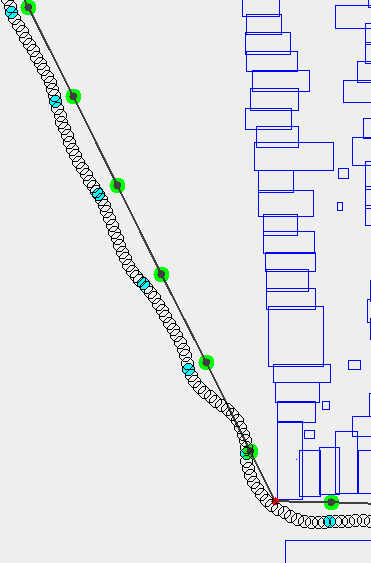
\includegraphics[width=\textwidth]{img/sf-wavy2}
        		\caption{}
        		\label{fig:sf-wavy2}
	\end{subfigure}
	\hfill
	\begin{subfigure}[t]{.4\textwidth}
        		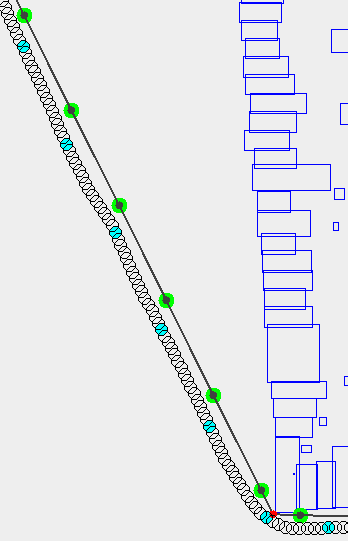
\includegraphics[width=\textwidth]{img/sf-wavy2b}
        		\caption{}
        		\label{fig:sf-wavy2b}
	\end{subfigure}	
	
        
    \caption[The effect of overlapping obstacles on oscillations in the trajectory]{Without overlapping the segments, oscillations tend to occur in the trajectory as seen in \ref{fig:sf-wavy2}. Even a small amount of overlap is an effective countermeasure as seen in \ref{fig:sf-wavy2b}.}
    \label{fig:sf-wavy}
\end{figure}
With the current algorithm there is a high performance cost involved with overlapping the segments. However, I do not believe this necessarily has to be the case. This is definitely something to look at in future work.

\subsection{Genetic Algorithm}
The genetic algorithm is the part of the thesis that got the least attention. This is mainly because the genetic algorithm itself is not an essential part of the trajectory planning algorithm. It is used to grow the convex safe region, and the current genetic algorithm does that well enough. Due to time constraints I have omitted detailed parameter tuning of this genetic algorithm.
\par
Either way, the genetic algorithm is very crude. A genetic algorithm was chosen to grow the convex safe region because it is a quick way to get a reasonably good result.  Since it never was the most pressing issue in the project, it never got replaced by a more refined algorithm (genetic or otherwise). 


